\chapter{Results}
In this chapter we present the outcome of using CNN's for recovering images from compressed measurements. First, we present the small network and its performance using both learning approaches: supervised and unsupervised. We present the training, test and validation error for LabelMe dataset \cite{LFWTech}. Afterwards, we also show the images from the test dataset and compare them against the ground truth in terms of PSNR and SSIM. The same data can be expected for the large network. Finally, we present the time measurement that our approach needs for fully reconstructing an image.  

\section{Small network}
The small network was describe in section \ref{ch:alphaNet}. It is not as deep as the large network and in the following we show its performance.
\subsection{Supervised training}
For supervised learning we train the network using compressed measurements generated with the constant matrix $\Phi$. The left figure in \ref{fig:alphaSupValidPSNRSSIM} shows the training of the network for 200 epochs. The blue line is the loss function MSE. The red solid line represents the PSNR on the whole training dataset whereas the red doted line represents the PSNR of the validation dataset. As it can been seen the PSNR on the validation set is not as high as in the training dataset but it is close. That means our network is not suffering from overfitting. On the right figure in \ref{fig:alphaSupValidPSNRSSIM} is the SSIM progress on the validation dataset over each epoch. Figure \ref{fig:alphaSupTestPSNRSSIM} shows the progress of PSNR and SSIM during training for the testing dataset. One can see that even though the difference is higher, approximately 4 dB, the reconstruction is considerably good. Higher values of PSNR and SSIM indicate better recovery quality. 
 
%\begin{figure}[!htb]
%\centering 
%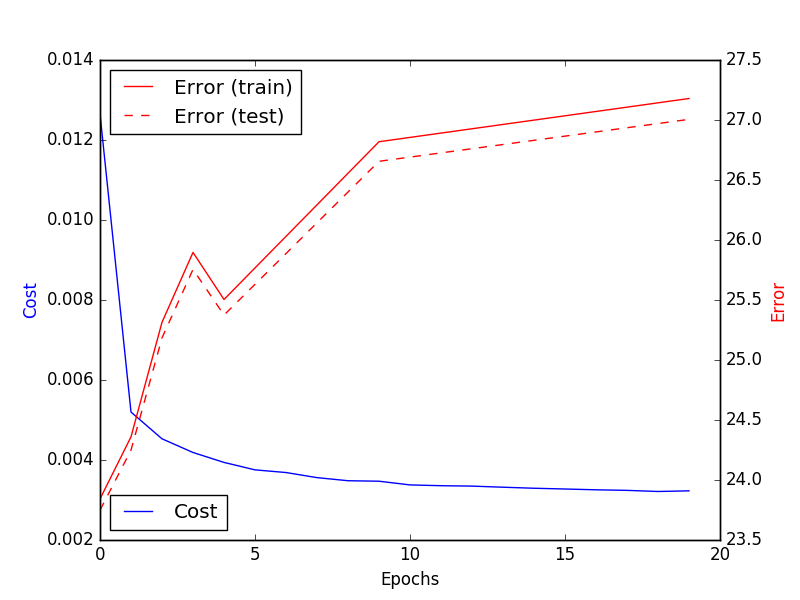
\includegraphics[scale=0.65]{alphaSup_PSNR_VALID_SET.png}
%\caption[PSNR validation progress during training of supervised alpha network]{PSNR progress over each epoch of supervised alpha network on validation dataset.}
%\label{fig:alphaSupValidPSNR} 
%\end{figure}  

%\begin{figure}[!htb] 
%\centering 
%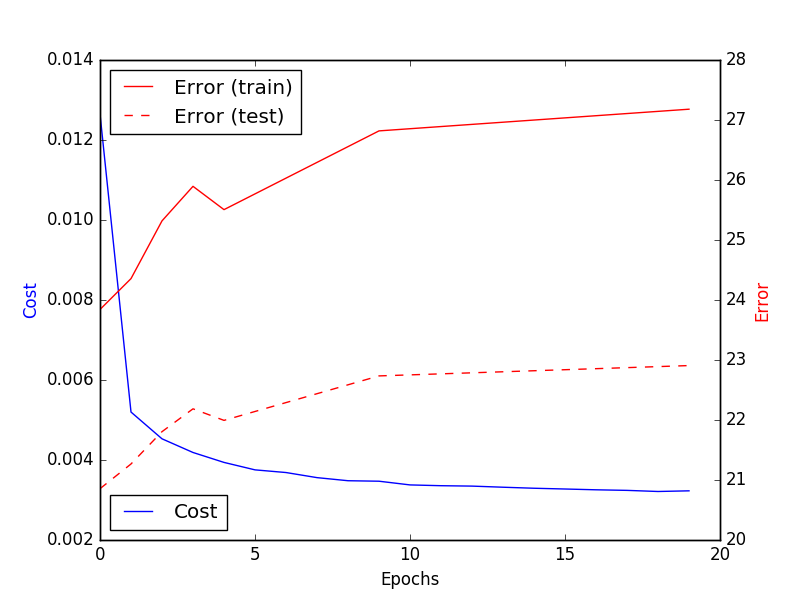
\includegraphics[scale=0.65]{alphaSup_PSNR_TEST_SET.png} 
%\caption[PSNR testing progress during training of supervised alpha network]{PSNR progress over each epoch of supervised alpha network on testing dataset.}
%\label{fig:alphaSupTestPSNR} 
%\end{figure}  

%\begin{figure}[!htb] 
%\centering 
%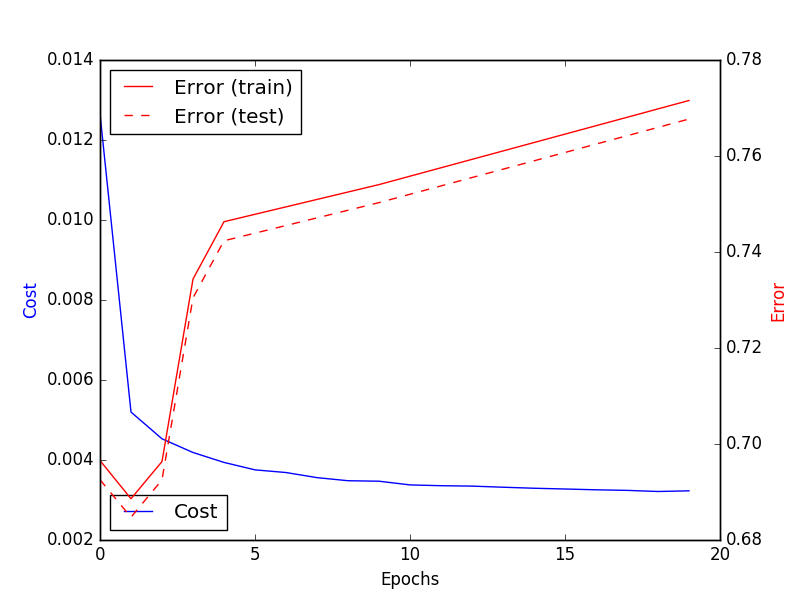
\includegraphics[scale=0.65]{alphaSup_SSIM_VALID_SET.png} 
%\caption[SSIM validation progress during training of supervised alpha network]{SSIM progress over each epoch of supervised alpha network on validation dataset.}
%\label{fig:alphaSupValidSSIM} 
%\end{figure}  

%\begin{figure}[!htb]
%\centering 
%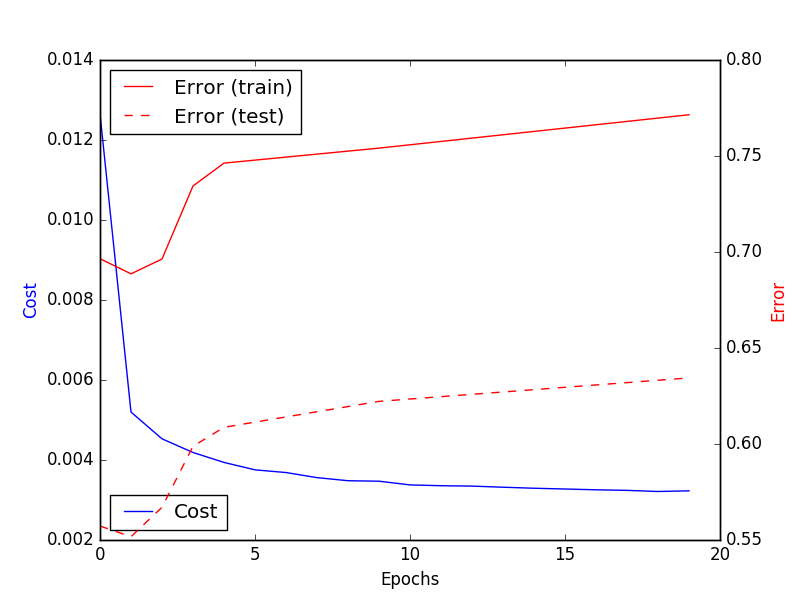
\includegraphics[scale=0.65]{alphaSup_SSIM_TEST_SET.png} 
%\caption[SSIM testing progress during training of supervised alpha network]{SSIM %progress over each epoch of supervised alpha network on testing dataset.}
%\label{fig:alphaSupTestSSIM} 
%\end{figure}  

\begin{figure}[!htb] 
\centering 
\subfloat[]{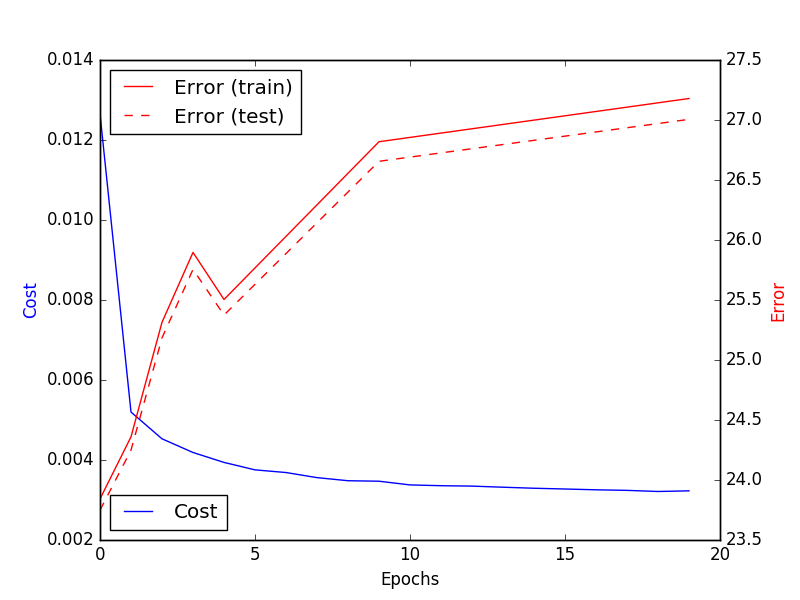
\includegraphics[width=3in]{alphaSup_PSNR_VALID_SET.png}} 
\subfloat[]{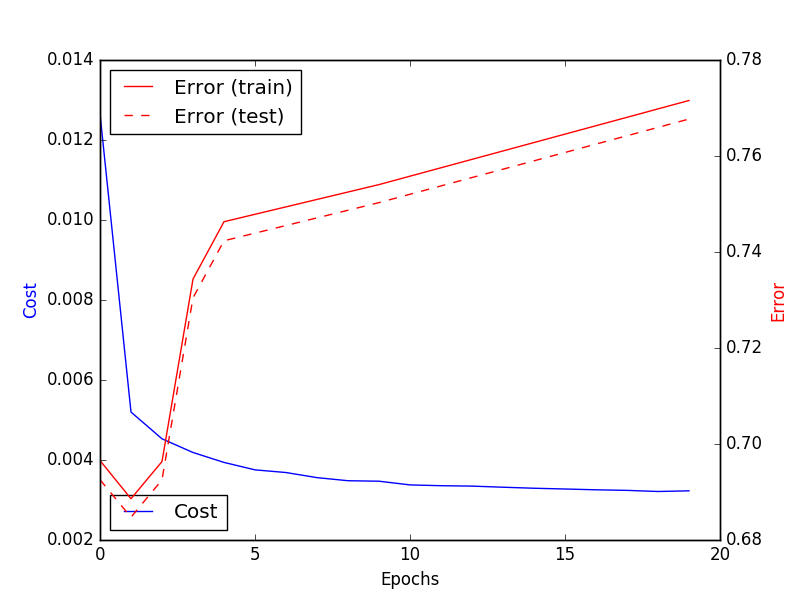
\includegraphics[width=3in]{alphaSup_SSIM_VALID_SET.png}} 
\caption[PSNR and SSIM validation progress during training of supervised small network]{\color{red}Error=PSNR \color{black}(left) and \color{red}Error=SSIM \color{black}(right) progress over each epoch of supervised small network on validation dataset.}
\label{fig:alphaSupValidPSNRSSIM} 
\end{figure}

\vspace{1cm}

\begin{figure}[!htb] 
\centering 
\subfloat[]{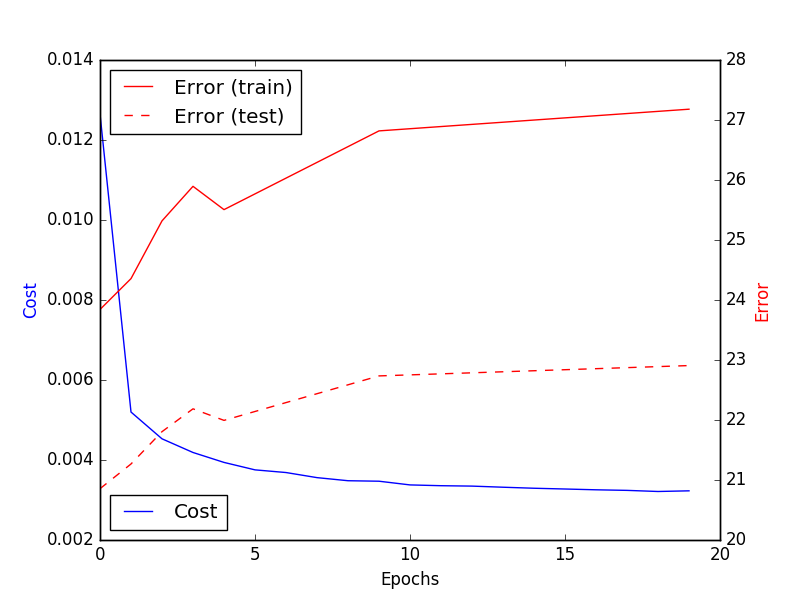
\includegraphics[width=3in]{alphaSup_PSNR_TEST_SET.png}} 
\subfloat[]{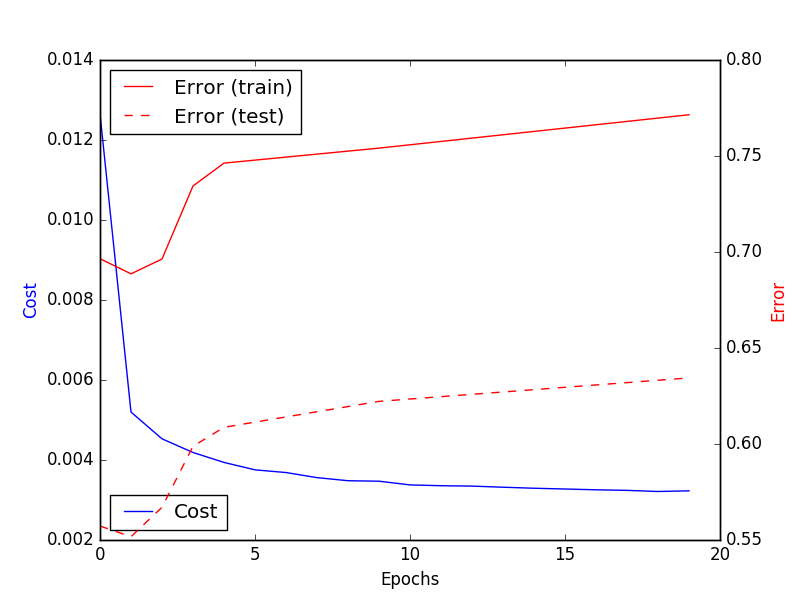
\includegraphics[width=3in]{alphaSup_SSIM_TEST_SET.png}} 
\caption[PSNR and SSIM testing progress during training of supervised small network]{\color{red}Error=PSNR \color{black}(left) and \color{red}Error=SSIM \color{black}(right) progress over each epoch of supervised small network on testing dataset.}
\label{fig:alphaSupTestPSNRSSIM} 
\end{figure}

%The reconstructed images from testing dataset using the supervised alpha network are shown in %figure \ref{fig:allReconAlphaSup}.

%\begin{figure}[tb] 
%\centering 
%\includegraphics[scale=1]{alphaSup_ReconAll.png} 
%\caption[Reconstructed testing images with supervised alpha network]{Ground truth, PSNR and %SSIM of reconstructed images from testing dataset using supervised alpha network.}
%\label{fig:allReconAlphaUnsup} 
%\end{figure}  

\FloatBarrier

\subsection{Unsupervised training}
For unsupervised learning the training data was not compressed beforehand. That is, the matrix $\Phi$ is intrinsically learned as the first layer of the network and the subsequent layers aim to reconstruct the image. Figure \ref{fig:alphaUnsupValidPSNRSSIM}  shows the progress of PSNR and SSIM over 200 epochs on validation datasets. Figure \ref{fig:alphaUnsupTestPSNRSSIM} depicts the same values for testing dataset using the same network. As it was expected learning the matrix $\Phi$ yielded better results. Namely, there was an increase of approximately 1.2 dB for PSNR and 0.02 for SSIM.    

%\begin{figure}[!htb] 
%\vspace{1.5cm}
%\centering 
%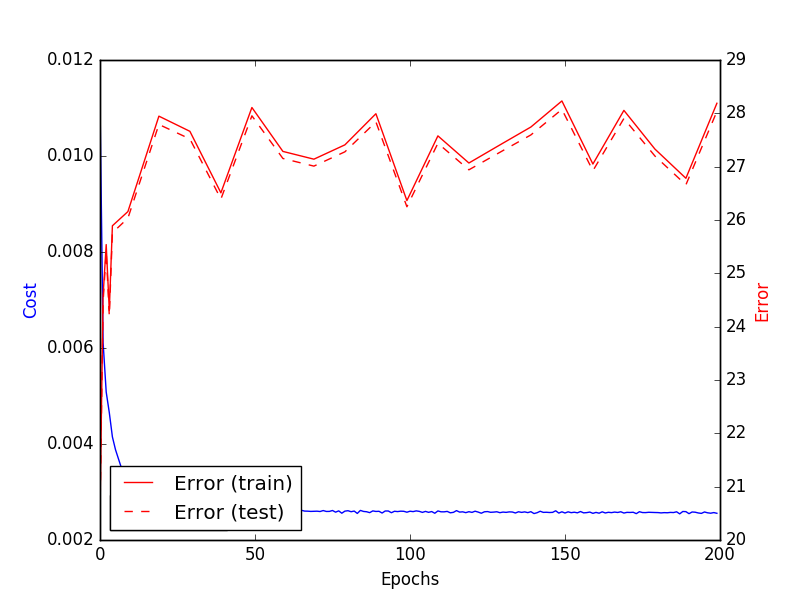
\includegraphics[scale=0.65]{alphaUnsup_PSNR_VALID_SET.png} 
%\caption[PSNR validation progress during training of unsupervised alpha network]{PSNR progress over each epoch of unsupervised alpha network on validation dataset.}
%\label{fig:alphaUnsupValidPSNR} 
%\end{figure}  
%
%\begin{figure}[!htb]
%\centering 
%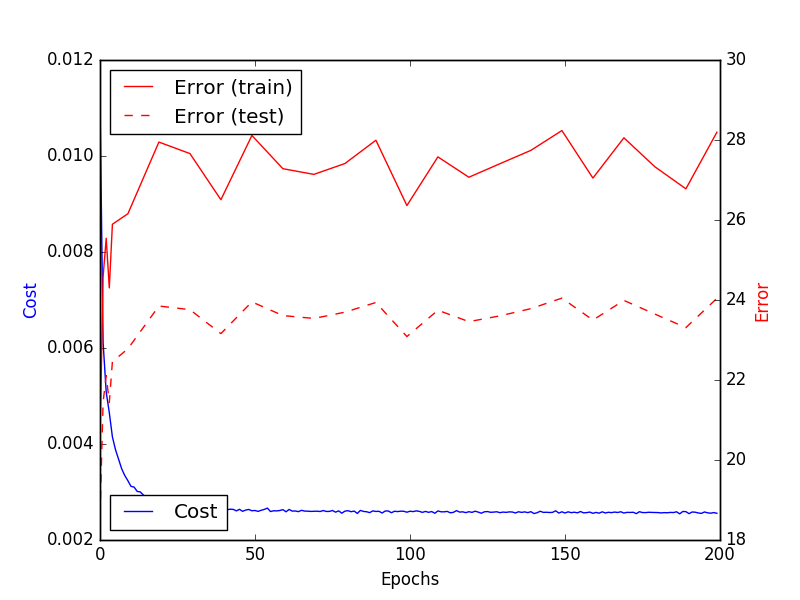
\includegraphics[scale=0.6]{alphaUnsup_PSNR_TEST_SET.png} 
%\caption[PSNR testing progress during training of unsupervised alpha network]{PSNR progress over each epoch of unsupervised alpha network on testing dataset.}
%\label{fig:alphaUnsupTestPSNR} 
%\end{figure}  
%
%\begin{figure}[!htb]
%\centering 
%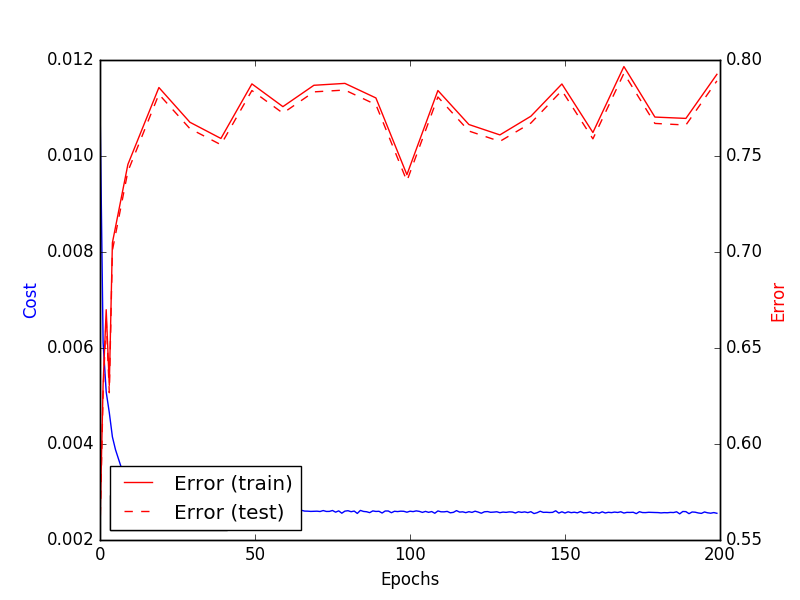
\includegraphics[scale=0.6]{alphaUnsup_SSIM_VALID_SET.png} 
%\caption[SSIM validation progress during training of unsupervised alpha network]{SSIM progress over each epoch of unsupervised alpha network on validation dataset.}
%\label{fig:alphaUnsupValidSSIM} 
%\end{figure}  
%
%\begin{figure}[!htb] 
%\centering 
%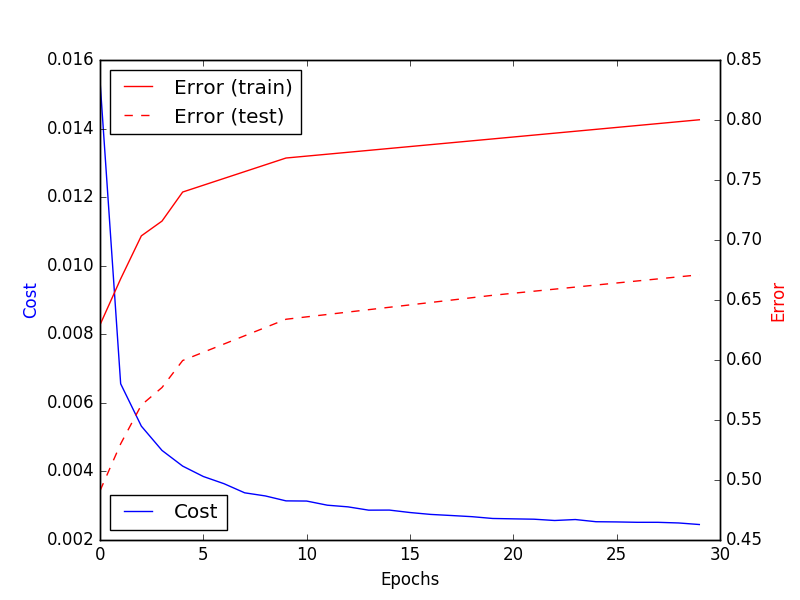
\includegraphics[scale=0.65]{alphaUnsup_SSIM_TEST_SET.png} 
%\caption[SSIM testing progress during training of unsupervised alpha network]{SSIM progress over each epoch of unsupervised alpha network on testing dataset.}
%\label{fig:alphaUnsupTestSSIM}
%\end{figure}  

\begin{figure}[!htb] 
\centering 
\subfloat[]{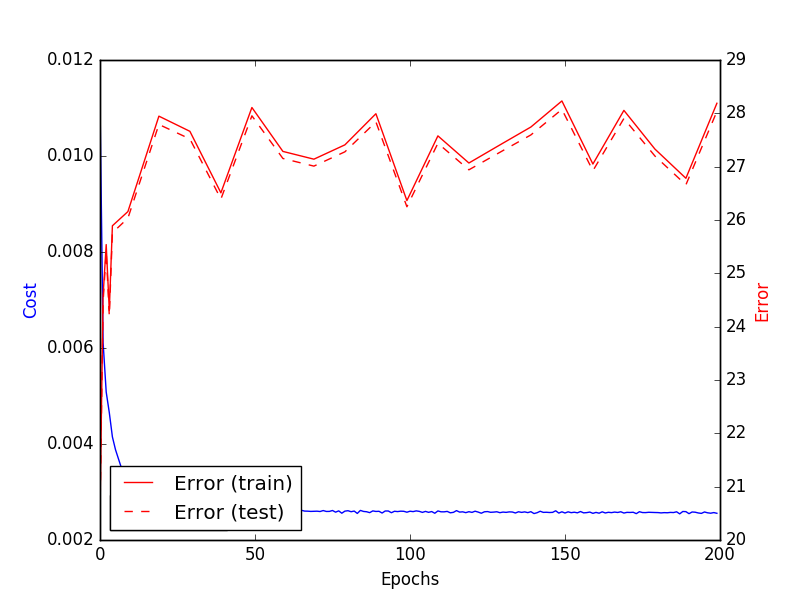
\includegraphics[width=3in]{alphaUnsup_PSNR_VALID_SET.png}} 
\subfloat[]{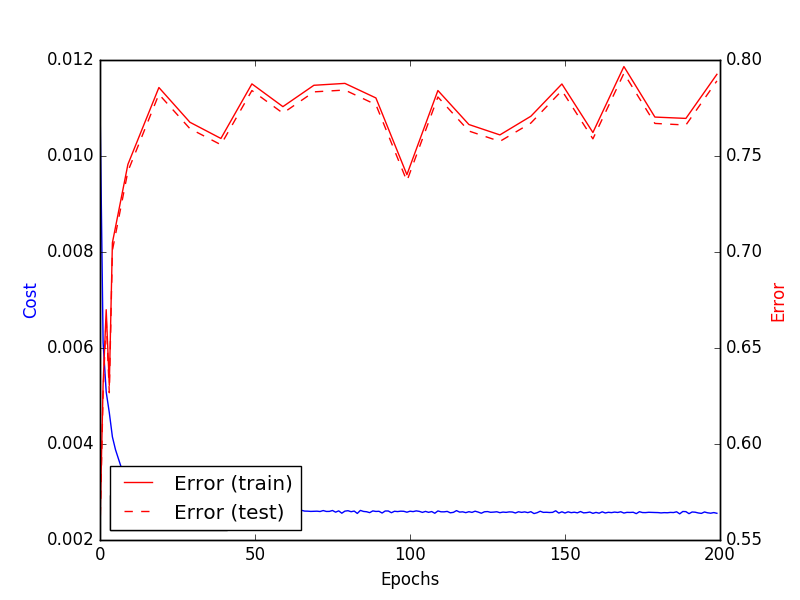
\includegraphics[width=3in]{alphaUnsup_SSIM_VALID_SET.png}} 
\caption[PSNR and SSIM validation progress during training of unsupervised small network]{\color{red}Error=PSNR \color{black}(left) and \color{red}Error=SSIM \color{black}(right) progress over each epoch of unsupervised small network on validation dataset.}
\label{fig:alphaUnsupValidPSNRSSIM} 
\end{figure}

\vspace{1cm}

\begin{figure}[!htb] 
\centering 
\subfloat[]{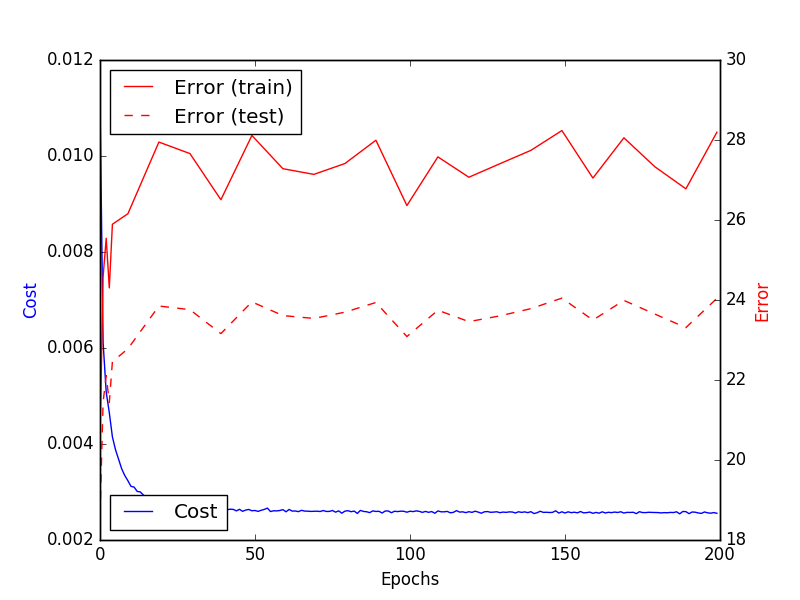
\includegraphics[width=3in]{alphaUnsup_PSNR_TEST_SET.png}} 
\subfloat[]{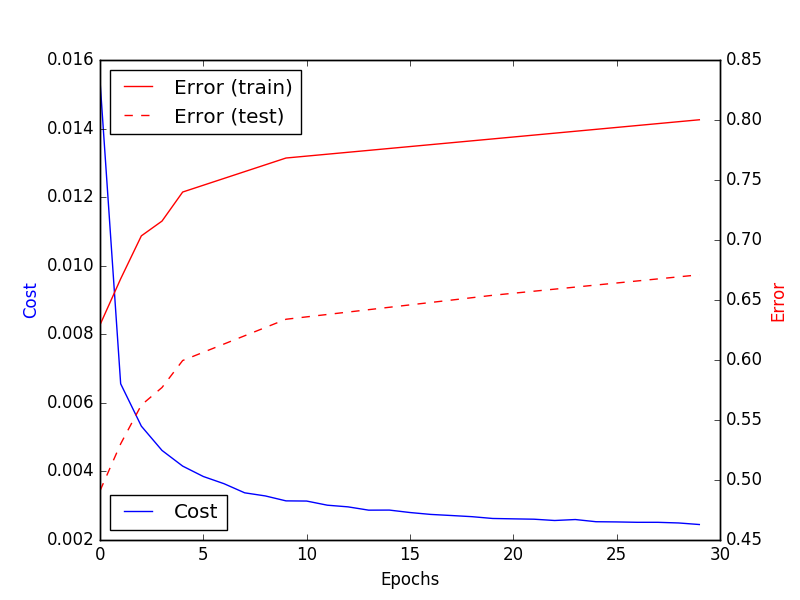
\includegraphics[width=3in]{alphaUnsup_SSIM_TEST_SET.png}} 
\caption[PSNR and SSIM testing progress during training of unsupervised small network]{\color{red}Error=PSNR \color{black}(left) and \color{red}Error=SSIM \color{black}(right) progress over each epoch of unsupervised small network on testing dataset.}
\label{fig:alphaUnsupTestPSNRSSIM} 
\end{figure}
%The reconstructed images from testing dataset using the unsupervised alpha network is shown %are figure \ref{fig:allReconAlphaUnsup}.

%\begin{figure}[tb] 
%\centering 
%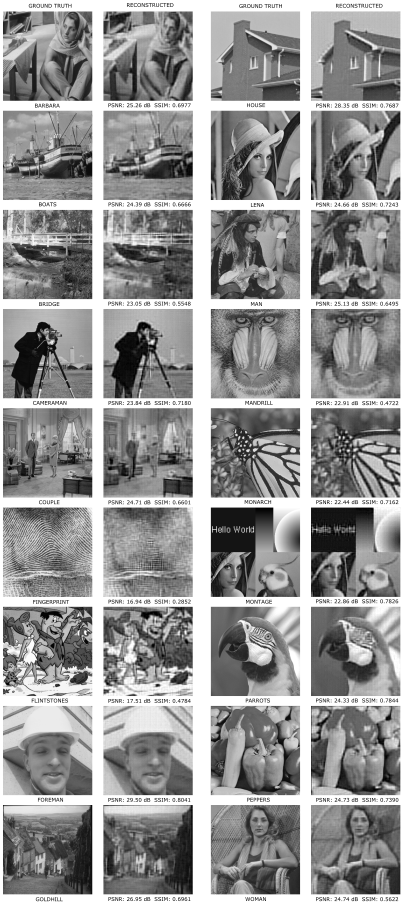
\includegraphics[scale=1]{alphaUnsup_ReconAll.png} 
%\caption[Reconstructed testing images with unsupervised alpha network]{Ground truth, PSNR and %SSIM of reconstructed images from testing dataset using unsupervised alpha network.}
%\label{fig:allReconAlphaUnsup} 
%\end{figure}  

\FloatBarrier



%%%%%%%%%%%%%%%%%%%%%%%%%%%%%%%%%%%BETA%%%%%%%%%%%%%%%%%%%%%%%%%%%%%%%%%%%%%%%%%%%%%%

\section{Large Network}
Large network is much deeper compared to small network. It was described in section \ref{ch:alphaNet} and in the following we present the results obtained during training.

\subsection{Supervised training}
This approach reconstructs images from compressed measurements. Like with small networks, we show the results after 200 trainign epochs. Figure \ref{fig:betaSupValidPSNRSSIM} shows the progress of PSNR and SSIM on the validation dataset. Large network, improves PSNR in approximately 1.1 dB and SSIM 0.03 with respect to small network. Figure \ref{fig:betaSupTestPSNRSSIM} shows the same information explained before on the testing datatset. 

%\begin{figure}[!htb]
%\centering 
%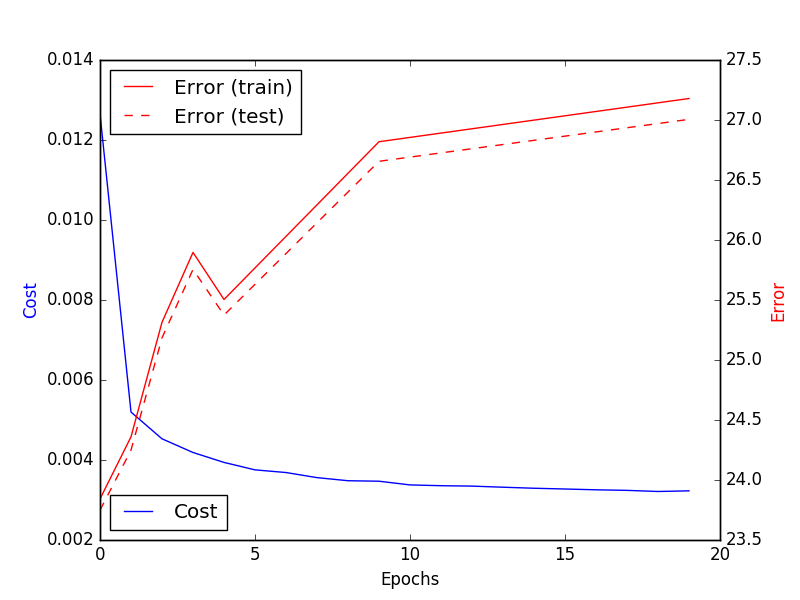
\includegraphics[scale=0.65]{betaSup_PSNR_VALID_SET.png} 
%\caption[PSNR validation progress during training of supervised large network]{PSNR progress over each epoch of supervised large network on validation dataset.}
%\label{fig:betaSupValidPSNR} 
%\end{figure}  
%
%\begin{figure}[!htb]
%\centering 
%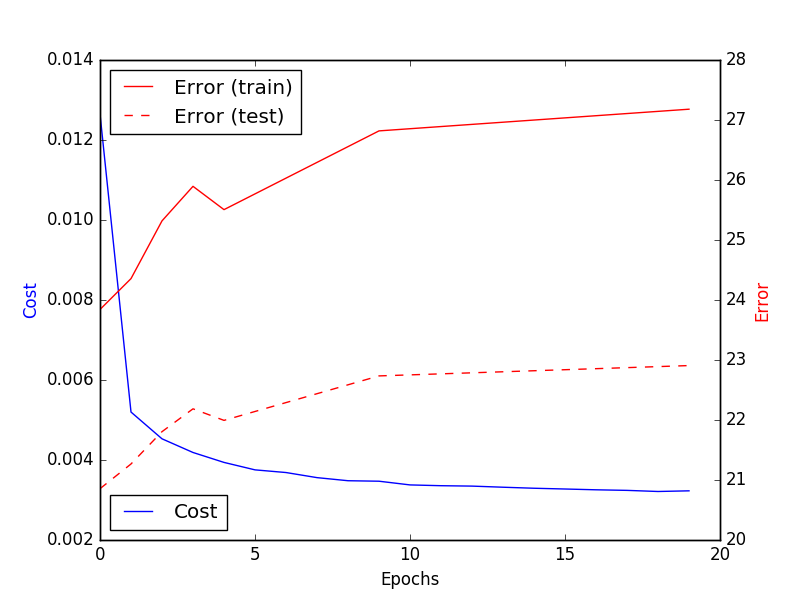
\includegraphics[scale=0.65]{betaSup_PSNR_TEST_SET.png} 
%\caption[PSNR testing progress during training of supervised large network]{PSNR progress over each epoch of supervised large network on testing dataset.}
%\label{fig:betaSupTestPSNR} 
%\end{figure}  
%
%\begin{figure}[!htb]
%\centering 
%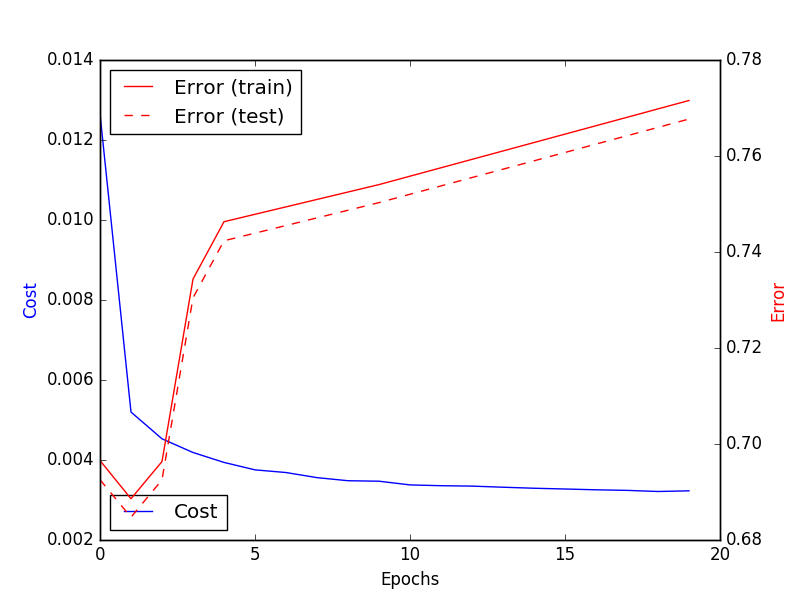
\includegraphics[scale=0.65]{betaSup_SSIM_VALID_SET.png} 
%\caption[SSIM validation progress during training of supervised large network]{SSIM progress over each epoch of supervised large network on validation dataset.}
%\label{fig:betaSupValidSSIM} 
%\end{figure}  
%
%\begin{figure}[!htb] 
%\centering 
%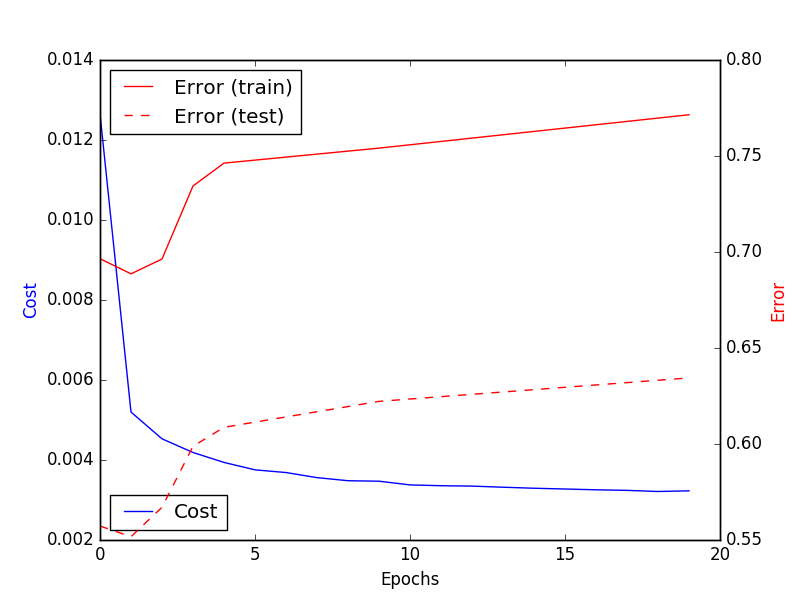
\includegraphics[scale=0.65]{betaSup_SSIM_TEST_SET.png} 
%\caption[SSIM testing progress during training of supervised large network]{SSIM progress over each epoch of supervised large network on testing dataset.}
%\label{fig:betaSupTestSSIM} 
%\end{figure}  

\begin{figure}[!htb] 
\centering 
\subfloat[]{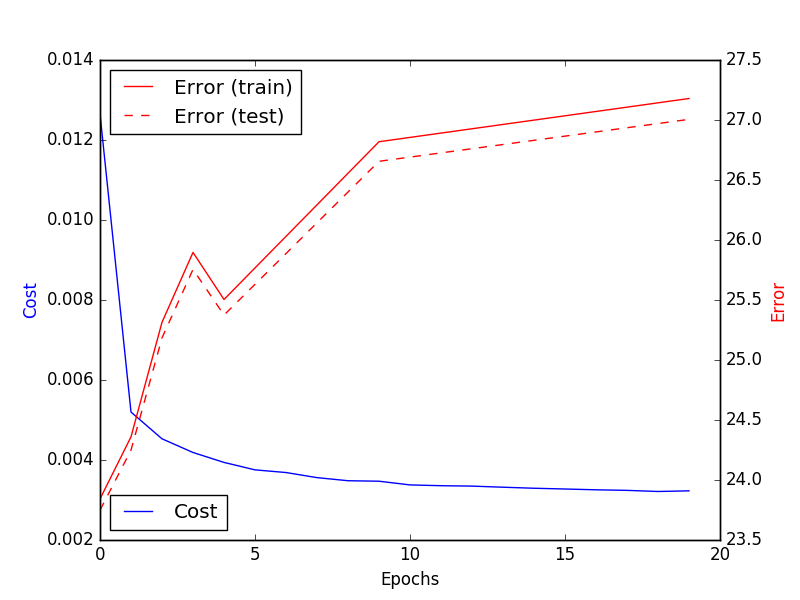
\includegraphics[width=3in]{betaSup_PSNR_VALID_SET.png}} 
\subfloat[]{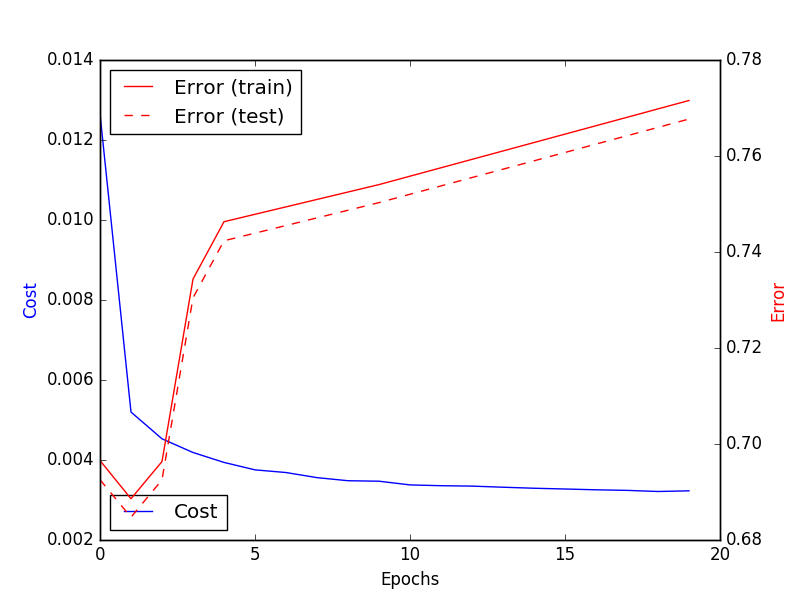
\includegraphics[width=3in]{betaSup_SSIM_VALID_SET.png}} 
\caption[PSNR and SSIM validation progress during training of supervised large network]{\color{red}Error=PSNR \color{black}(left) and \color{red}Error=SSIM \color{black}(right) progress over each epoch of supervised large network on validation dataset.}
\label{fig:betaSupValidPSNRSSIM} 
\end{figure}

\vspace{1cm}

\begin{figure}[!htb] 
\centering 
\subfloat[]{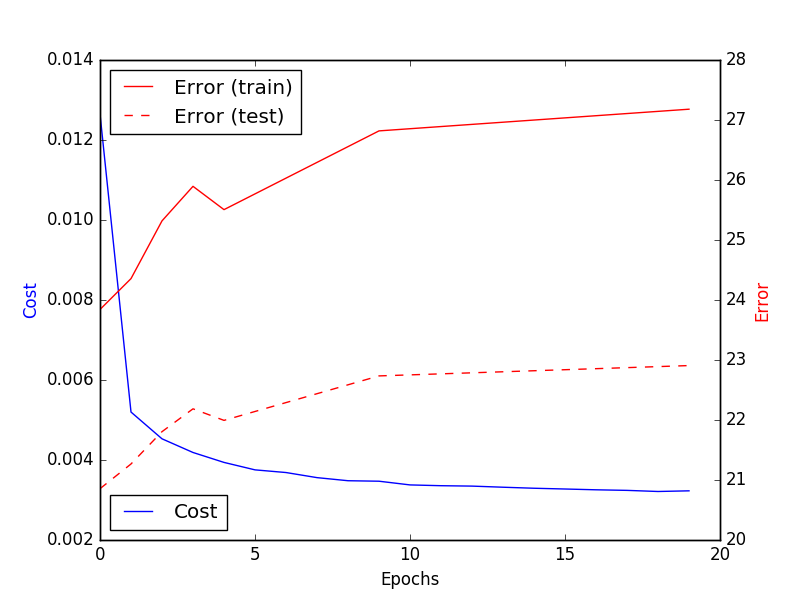
\includegraphics[width=3in]{betaSup_PSNR_TEST_SET.png}} 
\subfloat[]{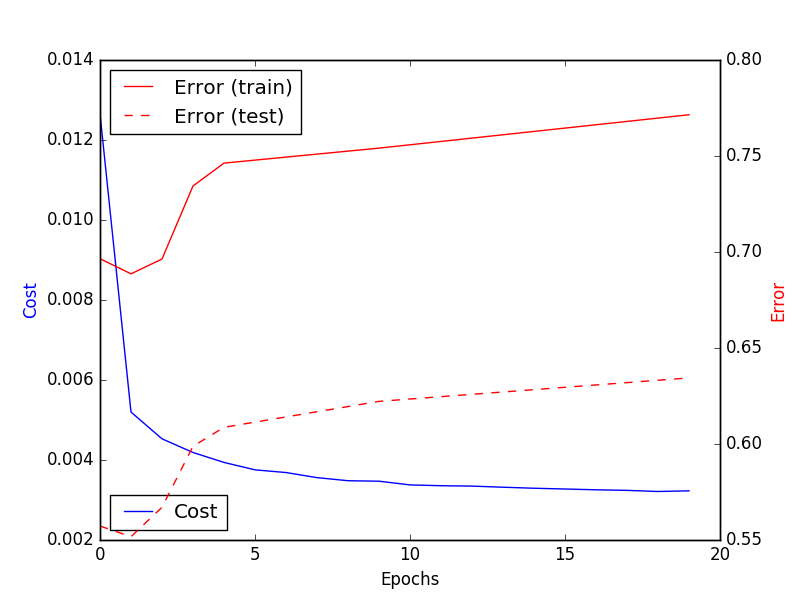
\includegraphics[width=3in]{betaSup_SSIM_TEST_SET.png}} 
\caption[PSNR and SSIM testing progress during training of supervised large network]{\color{red}Error=PSNR \color{black}(left) and \color{red}Error=SSIM \color{black}(right) progress over each epoch of supervised large network on testing dataset.}
\label{fig:betaSupTestPSNRSSIM} 
\end{figure}

\FloatBarrier

\subsection{Unsupervised training}
The traning for unsupervised learning uses the reshaped original images as its input. The compression phase is part of the network architecture and in the following we present the results of the training. Figure \ref{fig:betaUnsupValidPSNRSSIM} shows the progress in PSNR and SSIM over each epoch in the validation dataset and figure \ref{fig:betaUnsupTestPSNRSSIM} on the testing dataset. Compared to the small network it improves PSNR by 1 dB and SSIM by 0.04.     

%\begin{figure}[!htb]
%\vspace{2cm}
%\centering 
%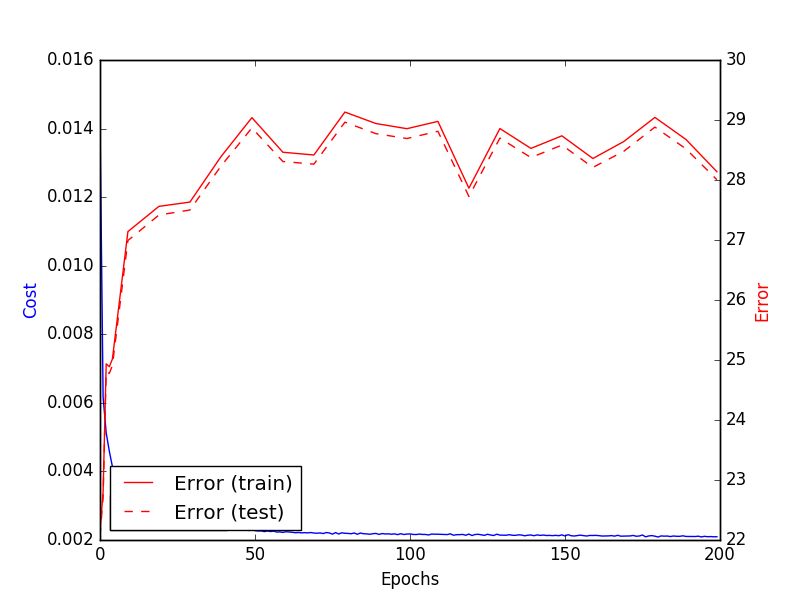
\includegraphics[scale=0.65]{betaUnsup_PSNR_VALID_SET.png} 
%\caption[PSNR validation progress during training of unsupervised large network]{PSNR progress over each epoch of unsupervised large network on validation dataset.}
%\label{fig:betaUnsupValidPSNR} 
%\end{figure}  

%\begin{figure}[!htb] 
%\centering 
%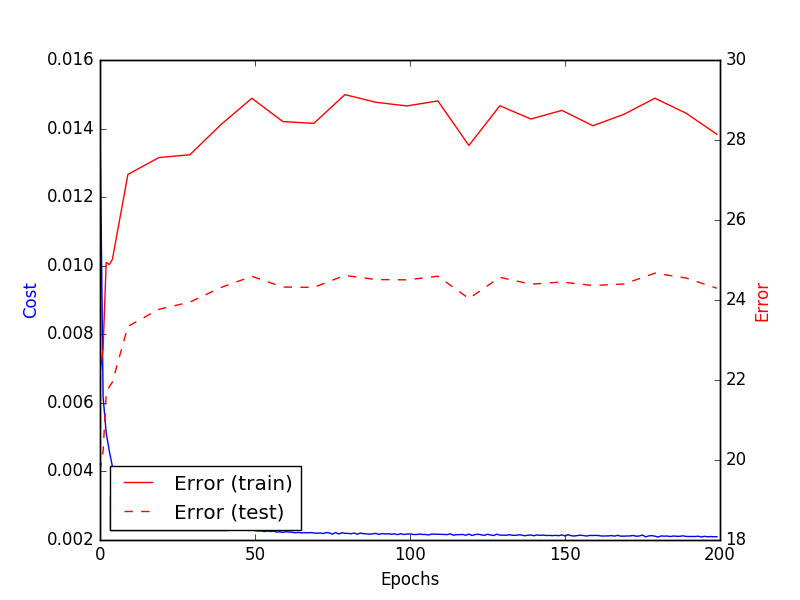
\includegraphics[scale=0.6]{betaUnsup_PSNR_TEST_SET.png} 
%\caption[PSNR testing progress during training of unsupervised large network]{PSNR progress over each epoch of unsupervised large network on testing dataset.}
%\label{fig:betaUnsupTestPSNR} 
%\end{figure}  

%\begin{figure}[!htb] 
%\centering 
%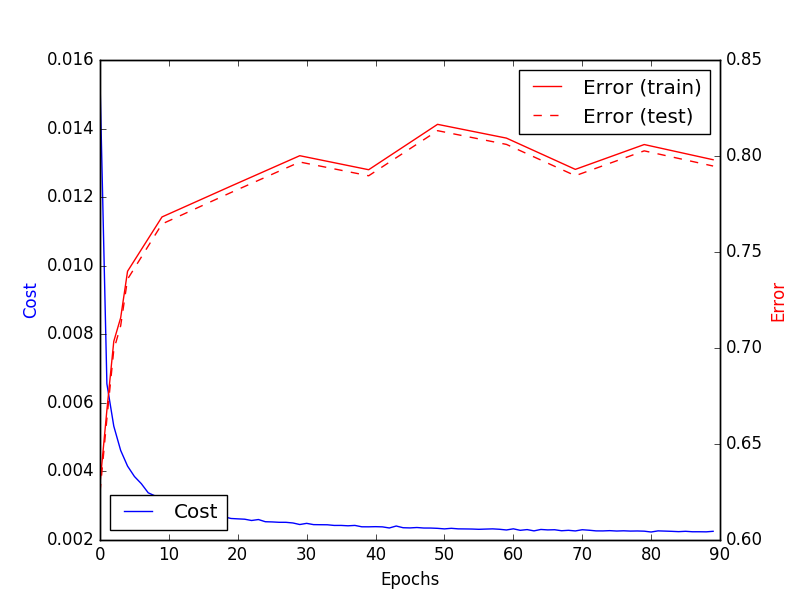
\includegraphics[scale=0.6]{betaUnsup_SSIM_VALID_SET.png} 
%\caption[SSIM validation progress during training of unsupervised large network]{SSIM progress over each epoch of unsupervised large network on validation dataset.}
%\label{fig:betaUnsupValidSSIM} 
%\end{figure}  

%\begin{figure}[!htb] 
%\centering 
%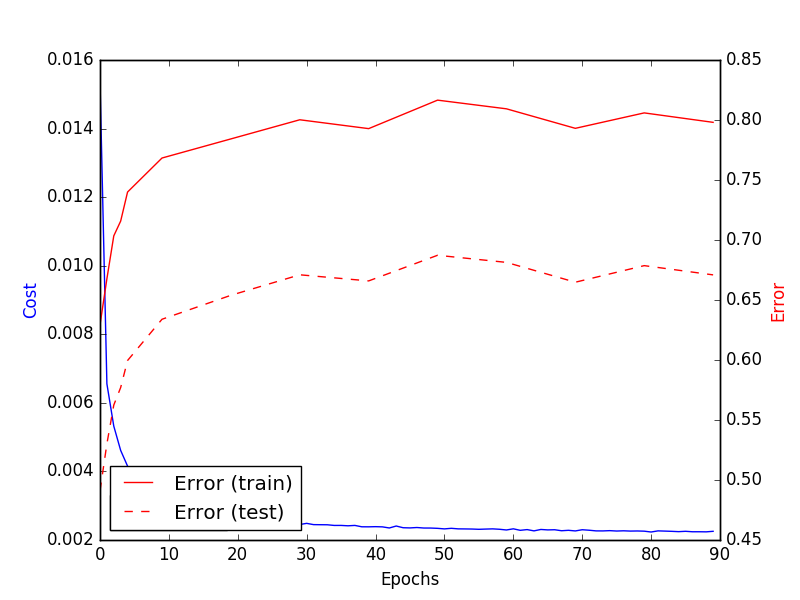
\includegraphics[scale=0.65]{betaUnsup_SSIM_TEST_SET.png} 
%\caption[SSIM testing progress during training of unsupervised large network]{SSIM progress over each epoch of unsupervised large network on testing dataset.}
%\label{fig:betaUnsupTestSSIM} 
%\end{figure}  

\begin{figure}[!htb] 
\centering 
\subfloat[]{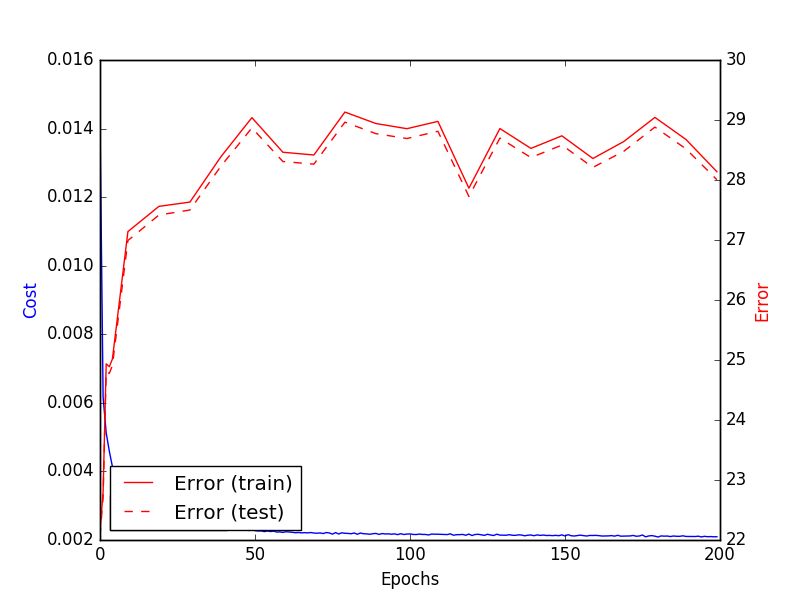
\includegraphics[width=3in]{betaUnsup_PSNR_VALID_SET.png}} 
\subfloat[]{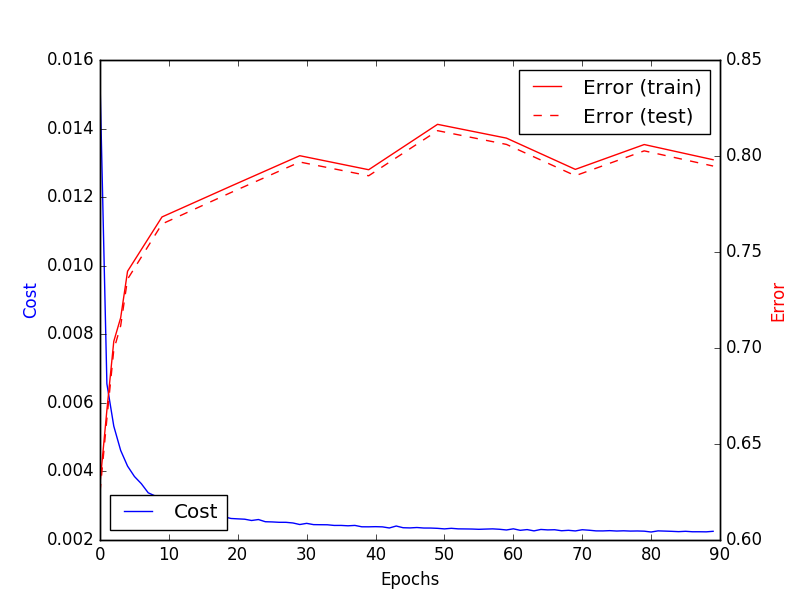
\includegraphics[width=3in]{betaUnsup_SSIM_VALID_SET.png}} 
\caption[PSNR and SSIM validation progress during training of unsupervised large network]{\color{red}Error=PSNR \color{black}(left) and \color{red}Error=SSIM \color{black}(right) progress over each epoch of unsupervised large network on validation dataset.}
\label{fig:betaUnsupValidPSNRSSIM} 
\end{figure}

\vspace{1cm}

\begin{figure}[!htb] 
\centering 
\subfloat[]{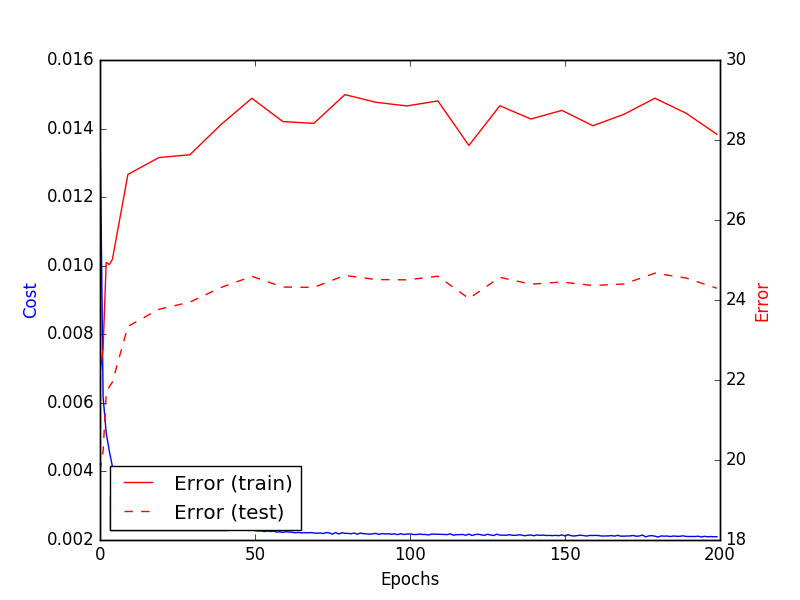
\includegraphics[width=3in]{betaUnsup_PSNR_TEST_SET.png}} 
\subfloat[]{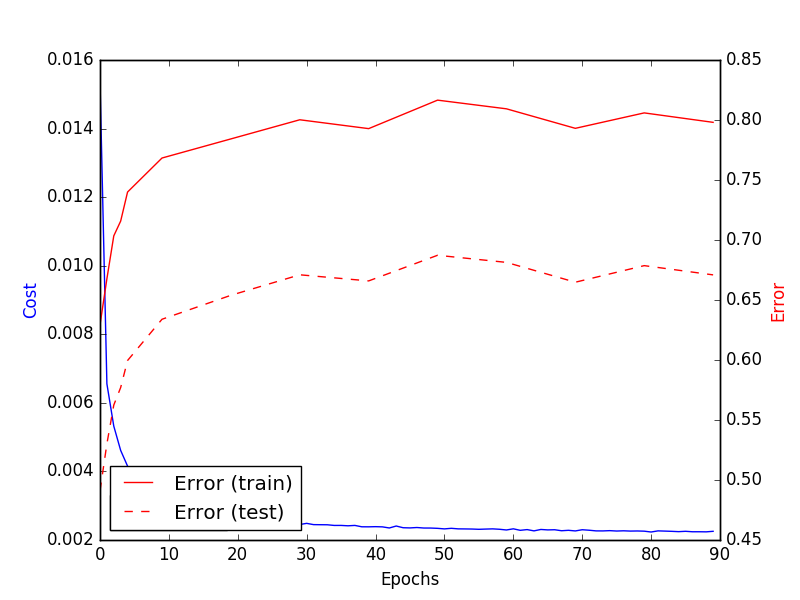
\includegraphics[width=3in]{betaUnsup_SSIM_TEST_SET.png}} 
\caption[PSNR and SSIM testing progress during training of unsupervised large network]{\color{red}Error=PSNR \color{black}(left) and \color{red}Error=SSIM \color{black}(right) progress over each epoch of unsupervised large network on testing dataset.}
\label{fig:betaUnsupTestPSNRSSIM} 
\end{figure}

\FloatBarrier

\newpage

\section{Results summary}

In this section we present a compendium of training and outcome of all proposed architecture networks for recovering the images. Table \ref{tab:summaryPSNR} shows PSNR for each dataset and Table \ref{tab:summarySSIM} does the same for SSIM. Additionaly, we add a column representing the denoised testing images using BM3D\cite{dabov2007image}. Using BM3D does not increase quality considereably but, it helps remove the block representaion introduced during preprocessing. It is clear that large network's performnce is better. 

\vspace{1cm}

\begin{table}[!htb]
\caption[Summary of PSNR for reconstructing networks]{Comparison of PSNR performance for each proposed network.}
\label{tab:summaryPSNR}
\begin{center}
\resizebox{\textwidth}{!}{
\begin{tabular}{l*{6}{c}r}
Network              & PSNR TRAINING & PSNR VALIDATION & PSNR TESTING & PSNR TESTING DENOISED\\
\hline
Small Supervised   & 26.47 dB & 26.31 dB & 22.37 dB & 22.54 dB\\
Small Unsupervised     & 28.19 dB & 28.03 dB & 24.02 dB & 24.24 dB\\
Large Supervised & 27.60 dB & 27.42 dB & 22.73 dB & 22.91 dB\\
Large Unsupervised & 29.14 dB & 28.96 dB & 24.63 dB & 24.77 dB\\
\bottomrule 
\end{tabular} }
\end{center}
\end{table}

\vspace{1.5cm}

\begin{table}[!htb]
\caption[Summary of SSIM for reconstructing networks]{Comparison of SSIM performance for each proposed network.}
\label{tab:summarySSIM}
\begin{center}
\resizebox{\textwidth}{!}{
\begin{tabular}{l*{6}{c}r}
Network              & SSIM TRAINING & SSIM VALIDATION & SSIM TESTING & PSNR TESTING DENOISED\\
\hline
Small Supervised   & 0.7507 & 0.7466 & 0.6062 & 0.6195\\
Small Unsupervised     & 0.7925 & 0.7891 & 0.6533 & 0.6715\\
Large Supervised & 0.7819 & 0.7781 & 0.6306 & 0.6381 \\
Large Unsupervised & 0.8155 & 0.8124 & 0.6873 & 0.6947\\
\bottomrule 
\end{tabular} }
\end{center}
\end{table}

\FloatBarrier

\newpage

\section{Reconstruction of testing dataset images}
In this section we show all testing images and the difference in reconstruction capabilities for each network. Each figure will provide a visual insight of the perfomance of each network. See figures \ref{fig:Recon1}, \ref{fig:Recon2}, \ref{fig:Recon3} and \ref{fig:Recon4}.  


\begin{figure}[!htb]
\vspace{1cm}
\centering 
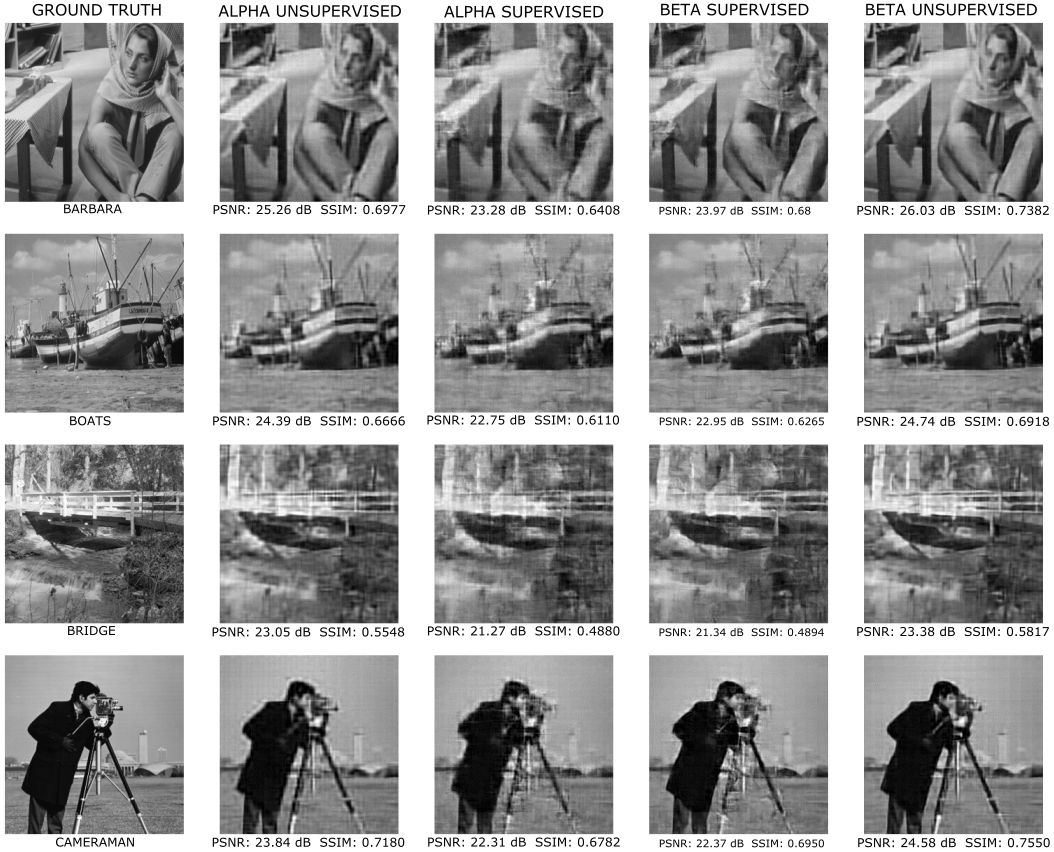
\includegraphics[width=\textwidth,height=\textheight,keepaspectratio=true]{ReaconIm1.png} 
\caption[Reconstructed testing images subset 1]{Reconstructed barbara, boats, bridge and cameraman compared against the ground truth, PSNR and SSIM.}
\label{fig:Recon1} 
\end{figure} 



\begin{figure}[!hb] 
\vspace{4.5cm}
\centering
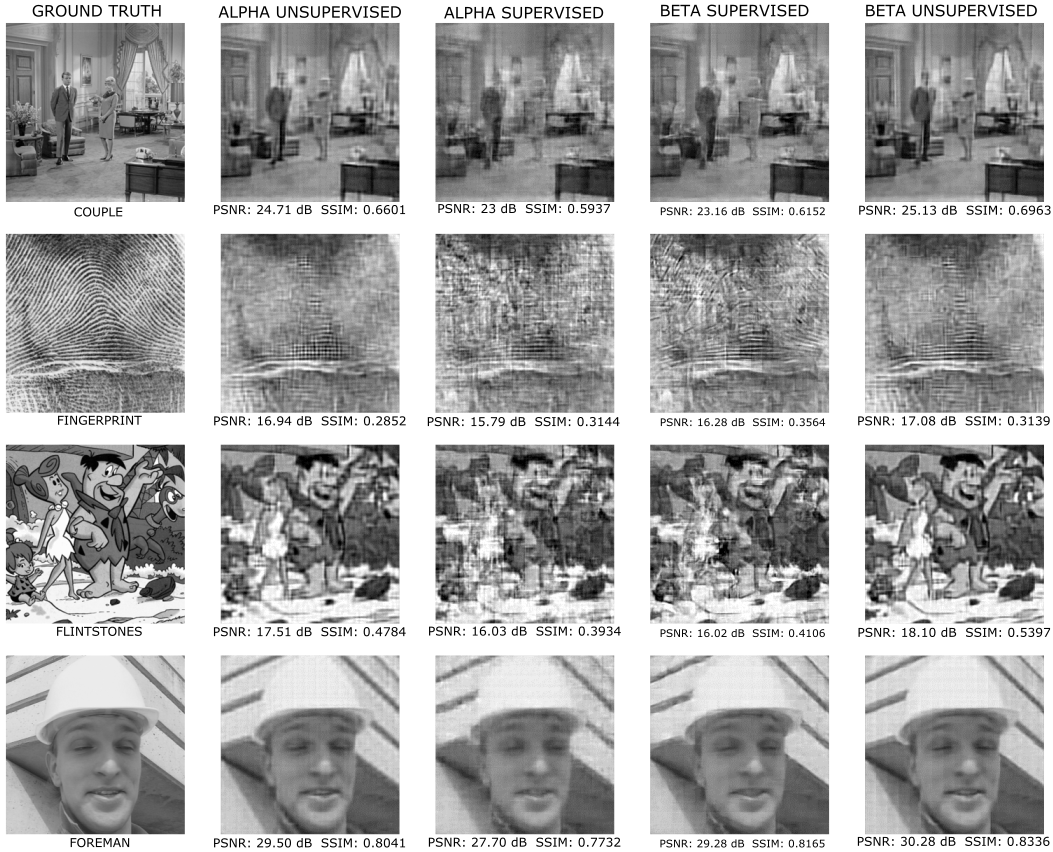
\includegraphics[width=\textwidth,height=\textheight,keepaspectratio=true]{ReaconIm2.png} 
\caption[Reconstructed testing images subset 2]{Reconstructed couple, fingerprint, flintstones and foreman images compared against the ground truth, PSNR and SSIM.}
\label{fig:Recon2} 
\end{figure}  



\begin{figure}[!htb]
\vspace{4.5cm}
\centering 
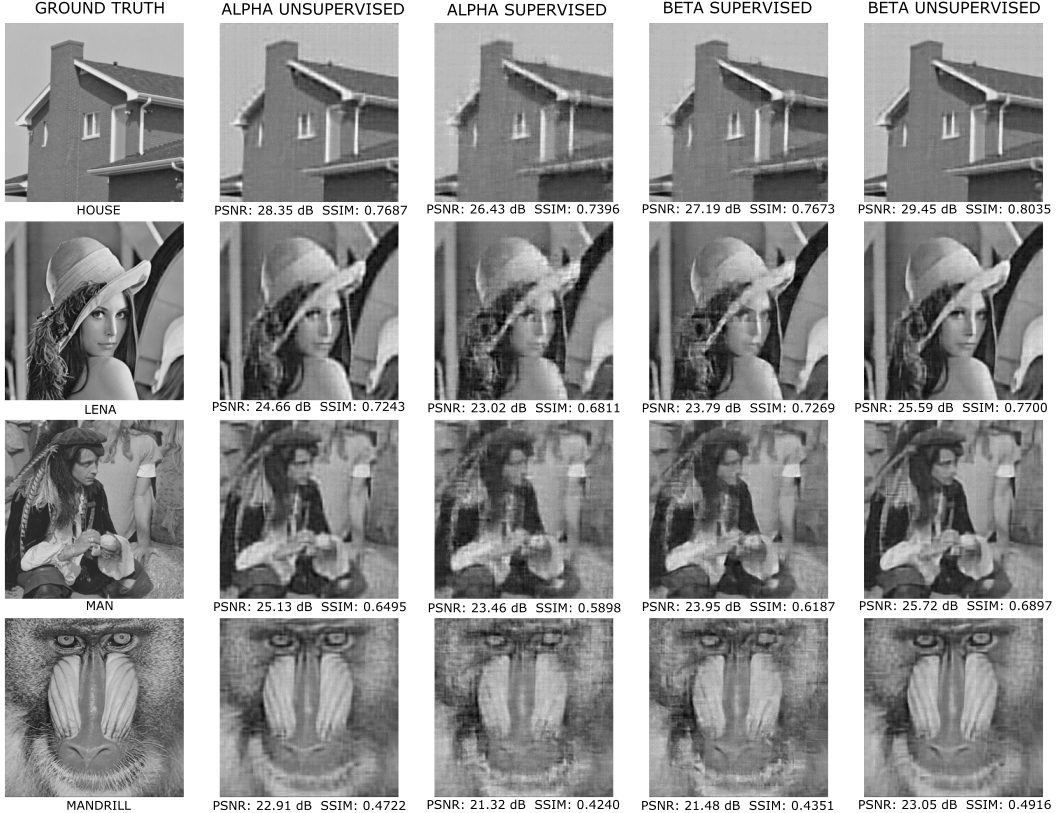
\includegraphics[width=\textwidth,height=\textheight,keepaspectratio=true]{ReaconIm3.png} 
\caption[Reconstructed testing images subset 3]{Reconstructed house, lena, man and mandrill images compared against the ground truth, PSNR and SSIM.}
\label{fig:Recon3} 
\end{figure} 

\begin{figure}[!htb] 
\vspace{3.5cm}
\centering 
%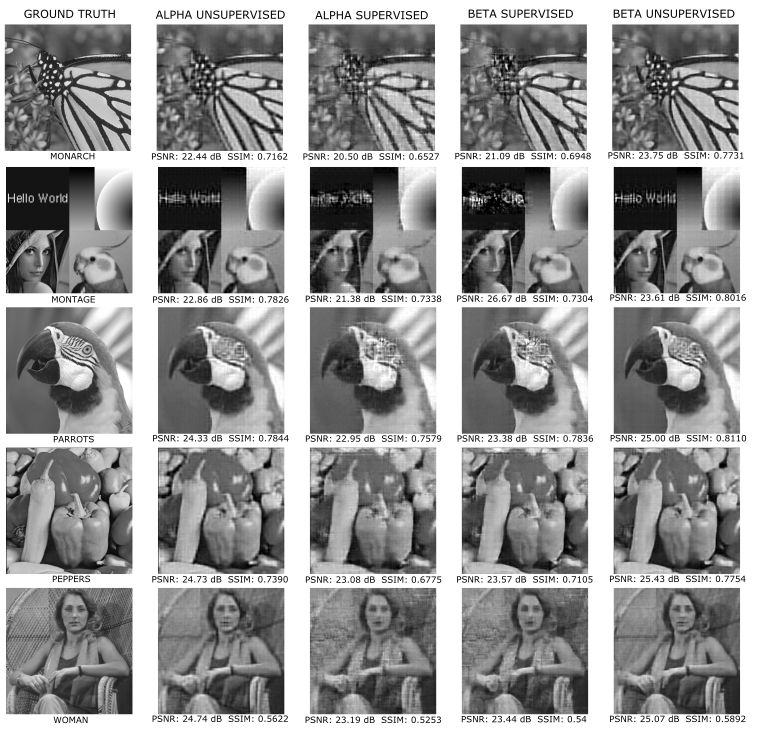
\includegraphics[width=15cm,height=21cm]{ReaconIm4.png} 
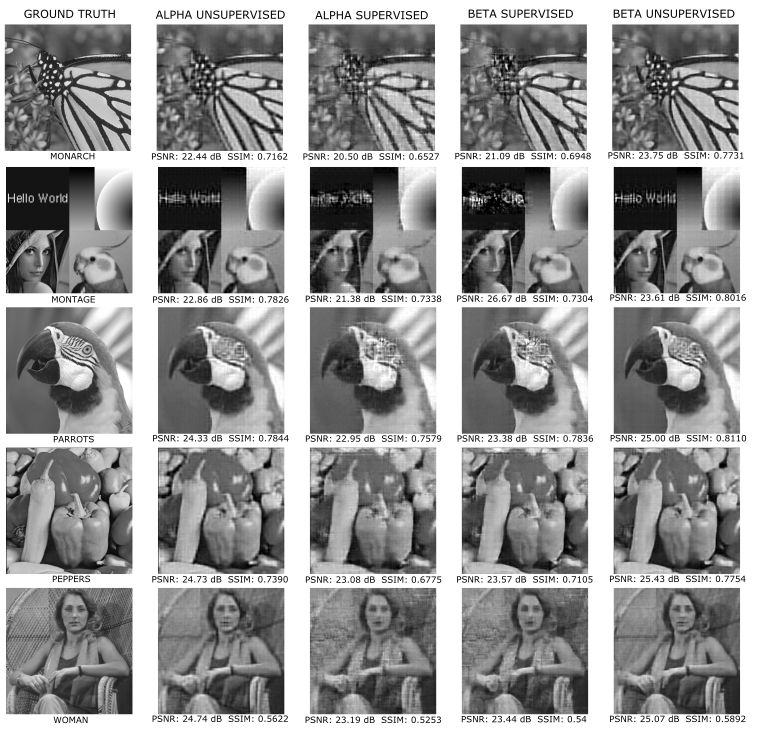
\includegraphics[width=\textwidth,height=\textheight,keepaspectratio=true]{ReaconIm4.png}
\caption[Reconstructed testing images subset 4]{Reconstructed monarch, montage, parrot, peppers and woman images compared against the ground truth, PSNR and SSIM.}
\label{fig:Recon4} 
\end{figure} 


\FloatBarrier
\section{Computational reconstruction time and quality comparison against traditional methods}
Table \ref{tab:summaryComp} compares our approach against some of the most recognized state-of-the-art algorithms for reconstruction. The table shows the average computational time and quality for the testing dataset. It is clear that using CNN's performs better in terms of quality and speed up. Particularly, using large network yields the best visual impact quality and speeds the recovery process more than 100x for NLR-CS, 90x for TVAL3 and 188x for D-AMP. It is important, however, to mention that the reported time for our approach is obtained using an Intel Xeon Core E5-2690 2.9GHz and the MATLAB code provided by their authors. Their code was adapted to have a fair comparison with our settings. That is using the same image size, compression rate and block size. The code implementing their proposed recovery algorithm was not touched. Our CNN's did not use the GPU for this test, we use the same CPU. Using GPU will considerably increase the speed-up even more.   

As an example, figure \ref{fig:Canman1} shows the the reconstruction of cameraman using several algorithms and our large network. While PSNR is similar among different approaches, the visual impact and SSIM of our network performs better.

\vspace{1.5cm}

%\begin{table}[!htb]
%\caption[Timing and quality metrics cameranman]{Comparison of reconstructing cameraman with several algorithms with subrate $\frac{1}{16}$.}
%\label{tab:summaryComp}
%\begin{center}
%%\resizebox{\textwidth}{!}{
%\begin{tabular}{l*{6}{c}r}
%Network              & TIME(sec) & PSNR & SSIM \\
%\hline
%TVAL3 & 122.12 & 24.15 dB & 0.6896\\
%NLR-CS & 200.95 & 18.51 dB & 0.5157\\
%D-AMP & 0.5871 & 24.19 dB & 0.5682\\
%Alpha Supervised   & 0.00251 & 22.31 dB & 0.6782\\
%Alpha Unsupervised     & 0.0095 & 23.84 dB & 0.718\\
%Beta Supervised & 0.00245 & 22.37 dB & 0.695 \\
%Beta Unsupervised & 0.0307 & 24.58 & 0.755\\
%\bottomrule 
%\end{tabular}%}
%\end{center}  
%\end{table}

\begin{table}[!htb]
\caption[Average time and quality metrics for testing dataset]{Comparison of reconstructing testing dataset with several algorithms with subrate $\frac{1}{16}$.}
\label{tab:summaryComp}
\begin{center}
%\resizebox{\textwidth}{!}{
\begin{tabular}{l*{6}{c}r}
Network              & TIME(sec) & PSNR & SSIM \\
\hline
TVAL3 & 255.50 & 23.04 dB & 0.5863\\
NLR-CS & 289.31 & 20.59 dB & 0.5575\\
D-AMP & 531.61 & 20.05 dB & 0.3628\\
Small Supervised   & 0.1654 & 22.39 dB & 0.6119\\
Small Unsupervised     & 0.3856 & 24.04 dB & 0.6595\\
Large Supervised & 0.6099 & 22.77 dB & 0.6360 \\
Large Unsupervised & 0.7612 & 25.18 & 0.6937\\
\bottomrule 
\end{tabular}%}
\end{center}  
\end{table}

\begin{figure}[!htb] 
\centering 
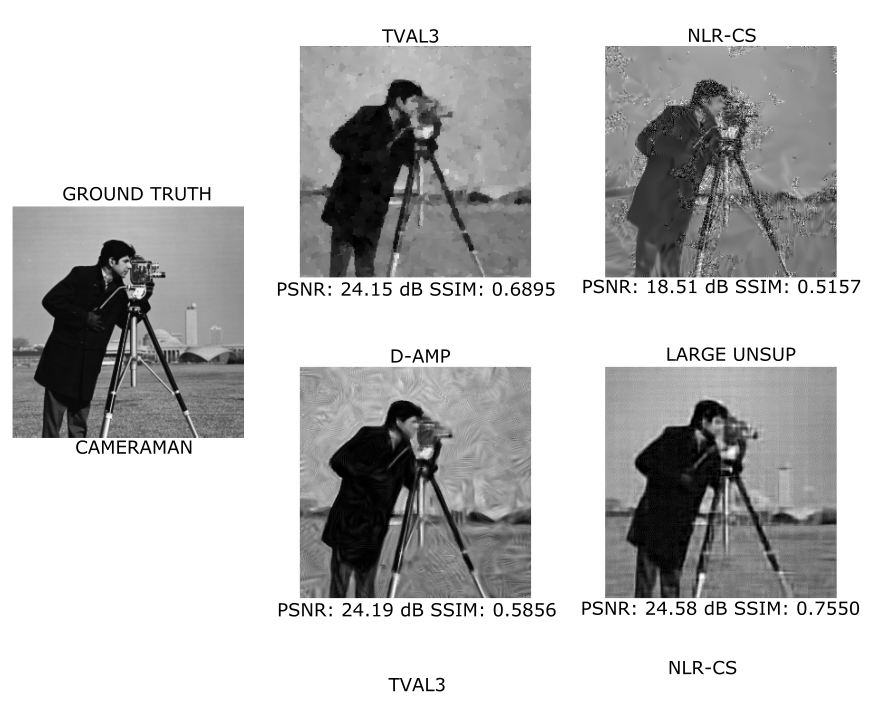
\includegraphics[width=\textwidth,height=\textheight,keepaspectratio=true]{CanMan.png}
\caption[Reconstructed cameraman with traditional methods]{Reconstructed cameraman using traditional CS algorithms and large network.}
\label{fig:Canman1} 
\end{figure} 

\FloatBarrier

\section{Reconstruction with alternate compression rates}

In this section we present the outcome when using subrates $\frac{1}{10}$, $C=10$ and $\frac{1}{8}$, $C=8$. We are only using large network because it produces the best results. As it will be seen, the gain in information is about 2 dB for PSNR and 0.05 for SSIM.  

\subsection{Compression rate 1/10}

Here we present the performance of our approach when reconstructing lena, barbara and woman. We also present the performance of the network during training on the testing dataset. See igure \ref{fig:trainTestsub1-10}. 

\begin{figure}[!htb] 
\centering 
\subfloat[]{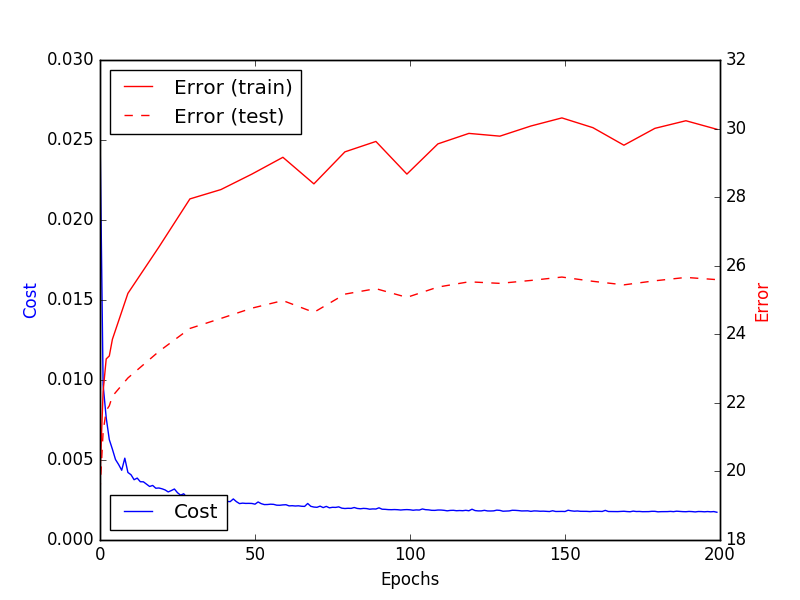
\includegraphics[width=3in]{PSNR_TEST_SET_sub1-10.png}} 
\subfloat[]{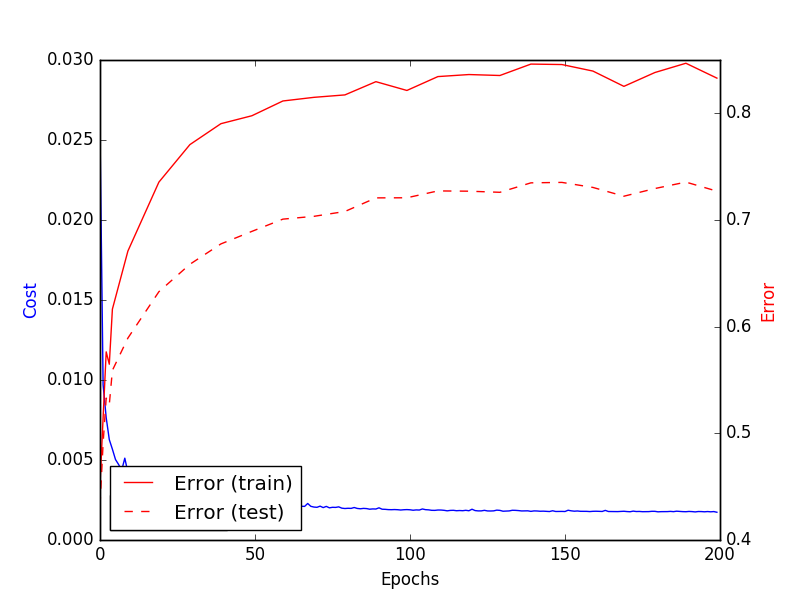
\includegraphics[width=3in]{SSIM_TEST_SET_sub1-10.png}} 
\caption[PSNR and SSIM traning for compression ratio 1/10.]{\color{red}Error=PSNR \color{black}(left) and \color{red}Error=SSIM \color{black}(right) development of testing dataset during training for compression ratio 1/10.}
\label{fig:trainTestsub1-10}
\end{figure}

Figure \ref{fig:ReconBLW} shows the reconstructed images with subrate $\frac{1}{10}$. Comparing against subrate $\frac{1}{16}$ there is an expected improvemented and the visual impact was also well preserved. We show this result so is easy to evalute the trade-off between quality and compression ratio. 

%\begin{figure}[!htb] 
%\centering 
%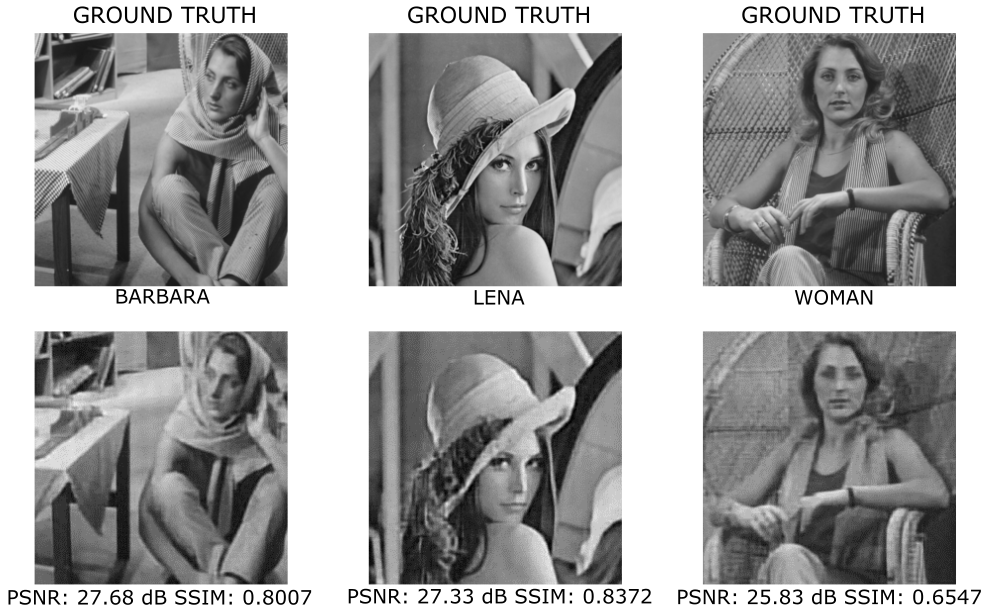
\includegraphics[width=\textwidth,height=\textheight,keepaspectratio=true]{ReconBLW_1-10.png}
%\caption{Reconstructed barbara, lena and woman with subrate 1/10.}
%\label{fig:ReconBLW_1-10} 
%\end{figure}

\FloatBarrier

\subsection{Compression rate 1/8}

In this section we introduce the same results as before for a compression ration of $\frac{1}{8}$. Figure \ref{fig:trainTestsub1-8} shows training phase. 

\begin{figure}[!htb] 
\centering 
\subfloat[]{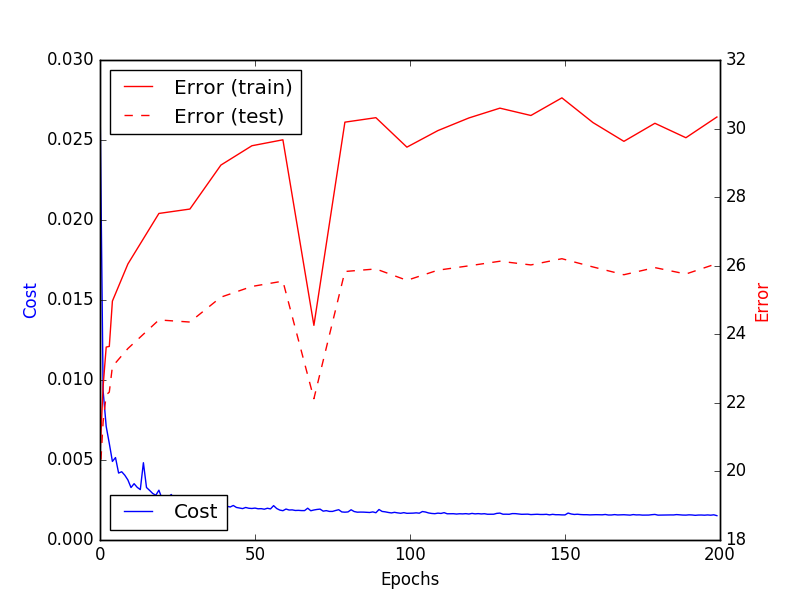
\includegraphics[width=3in]{PSNR_TEST_SET_sub1-8.png}} 
\subfloat[]{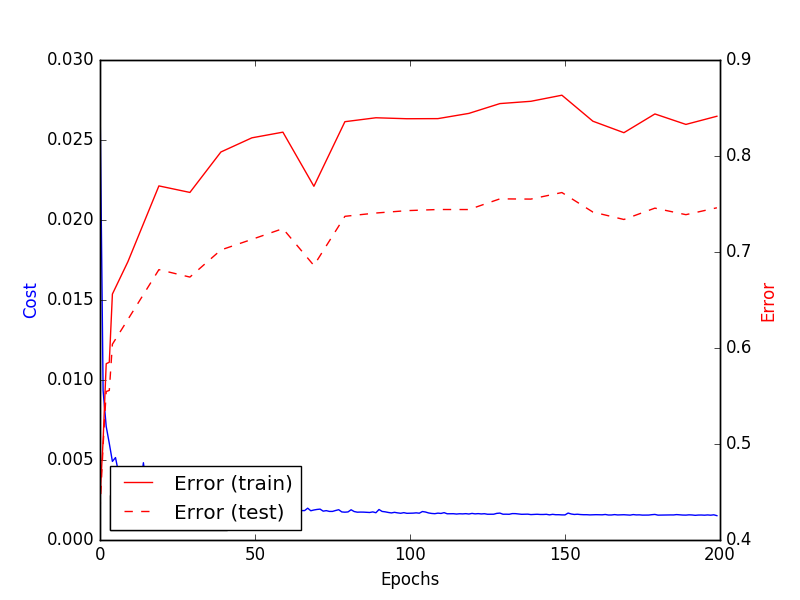
\includegraphics[width=3in]{SSIM_TEST_SET_sub1-8.png}} 
\caption[PSNR and SSIM traning for compression ratio 1/8.]{\color{red}Error=PSNR \color{black}(left) and \color{red}Error=SSIM \color{black}(right) development of testing dataset during training for compression ratio 1/8.}
\label{fig:trainTestsub1-8}
\end{figure}

\FloatBarrier

Figure \ref{fig:ReconBLW} shows the reconstructed images with both subrates. It is also evident that decreasing the compression ratio also helps getting rid off the block effect which would not requiere any denoising. This is also another feature of our network proposal.  

\begin{figure}[!htb] 
\centering 
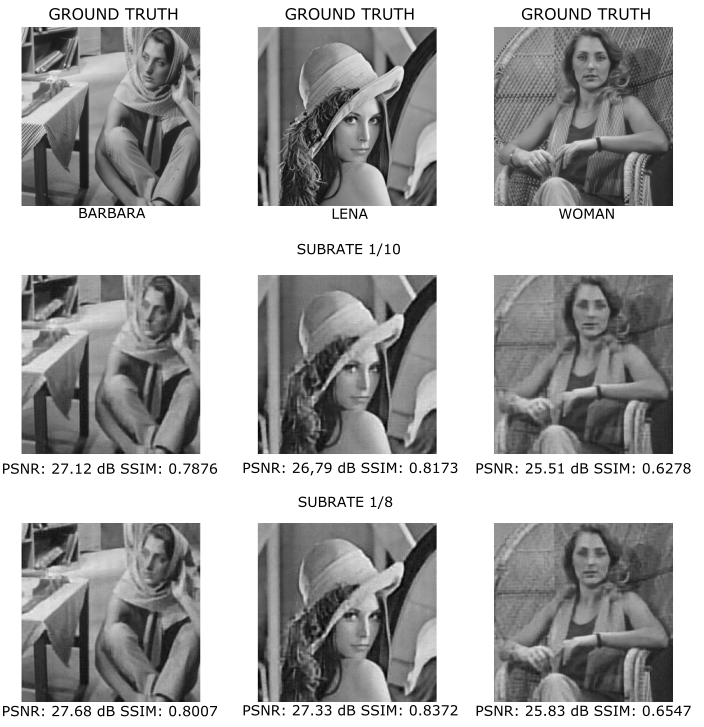
\includegraphics[width=\textwidth,height=\textheight,keepaspectratio=true]{ReconBLW.png}
\caption{Reconstructed barbara, lena and woman using subrates 1/8 and 1/10.}
\label{fig:ReconBLW} 
\end{figure}


